% Input common header
\documentclass[xcolor=dvipsnames]{beamer}

\usecolortheme[named=Blue]{structure}
\setbeamertemplate{itemize items}[circle]

\usepackage{smartdiagram}


\author{Dr. Paul Larsen}
\date{\today}


\title{Risk and Artificial Intelligence: Credit Scoring in Practice}
\begin{document}
\maketitle

\begin{frame}{Operational Risk in Credit Scoring}
    \framesubtitle{Model Risk and Process Risk}
    \begin{block}{The AI Act}
        \begin{quote}
            Manage model risk: Don't let the data-fed models speak nonsense
        \end{quote}
    \end{block}
    \begin{block}{The Supervisory Requirements for IT in German Asset Managers}
        \begin{quote}
            Manage process risk: Automate everything that makes sense
        \end{quote}
    \end{block}
\end{frame}

\begin{frame}
\frametitle{Manage Model Risk}
\framesubtitle{Don't outsource thinking to algorithms}
    \begin{center}
\smartdiagramset{
	back arrow disabled=true,
}
\smartdiagram[flow diagram:verticall]{Reality,
  Data, AI}
    \end{center}
\end{frame}

\begin{frame}{Manage Model Risk}
    \framesubtitle{Example of credit scoring for loans}

    \href{https://github.com/munichpavel/risk-ai-workshop/blob/main/notebooks/data/default.csv}{Artificial credit scoring data sample}:
    \newline\newline
    \begin{tabular}{rrr}
    \toprule
    default & gender & occupation \\
    \midrule
    0 & 1 & 1 \\
    0 & 0 & 1 \\
    0 & 0 & 1 \\
    1 & 0 & 1 \\
    1 & 0 & 1 \\
    1 & 0 & 0 \\
    0 & 1 & 0 \\
    1 & 1 & 0 \\
    \bottomrule
\end{tabular}
    \newline
    \newline
    \textbf{gender}: 0 for female, 1 for male \footnote{
        Some current and future credit data will likely have a non-binary gender category.
    } \newline
    \textbf{occupation}: 0 for education, 1 for health \newline
    \textbf{activity}: 0 for low account activity, 1 for high account activity \newline
    \textbf{default}: 0 for no-default, 1 for default \newline
\end{frame}

\begin{frame}{Manage Model Risk}
    \framesubtitle{Simpson's paradox again}
    Correlations with default:
    \newline
    \newline
    \begin{tabular}{llrr}
 & pair & pearson\_r & p\_value \\
0 & ('gender', 'default') & -0.097396 & 0.000000 \\
1 & ('occupation', 'default') & -0.221915 & 0.000000 \\
2 & ('activity', 'default') & 0.953242 & 0.000000 \\
\end{tabular}
\newline
    \newline
    Selected sub-population default rates:
    \newline
    \newline
    \begin{tabular}{lrr}
\toprule
population &   female &     male \\
\midrule
     total & 0.395094 & 0.302303 \\
 education & 0.449205 & 0.461679 \\
    health & 0.228145 & 0.245443 \\
\bottomrule
\end{tabular}
\newline

\end{frame}

\begin{frame}{Manage Model Risk}
    \framesubtitle{Spurious correlations aren't the only ones to fear}
    \begin{itemize}
        \item Colliders from target to a feature(s)
        \item \href{https://en.wikipedia.org/wiki/Leakage\_(machine\_learning)}{Data leakage}
    \end{itemize}

\end{frame}

\begin{frame}{Manage Model Risk}
    \framesubtitle{Collider risk: causality knows direction, correlation doesn't}
    What if we had causal graph with features \textrm{collider}$, \textrm{other}$ and target \textrm{default}?
    \newline
    \begin{figure}[ht]
        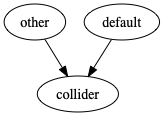
\includegraphics[height=0.5\textheight]{graphics/default_fork}
    \end{figure}
\end{frame}

\begin{frame}{Manage Model Risk}
    \framesubtitle{Data leakage risk: know your process, know your data}
    How I understood credit default pre-practical-experience
    \newline
    \begin{figure}[ht]
        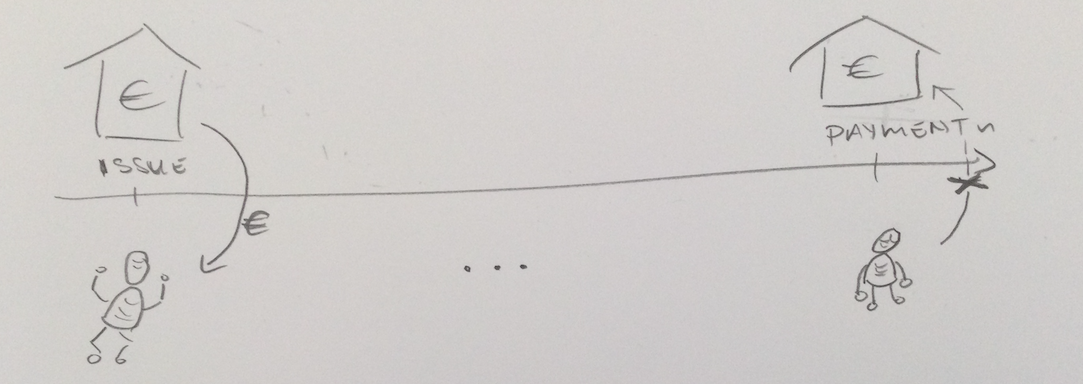
\includegraphics[height=0.5\textheight]{graphics/default-process-start}
    \end{figure}

\end{frame}

\begin{frame}{Manage Model Risk}
    \framesubtitle{Data leakage risk II: know your process, know your data}
    How credit default really\footnote{
        more accurately, a less violent projection of reality
    } happens
    \newline
    \begin{figure}[ht]
        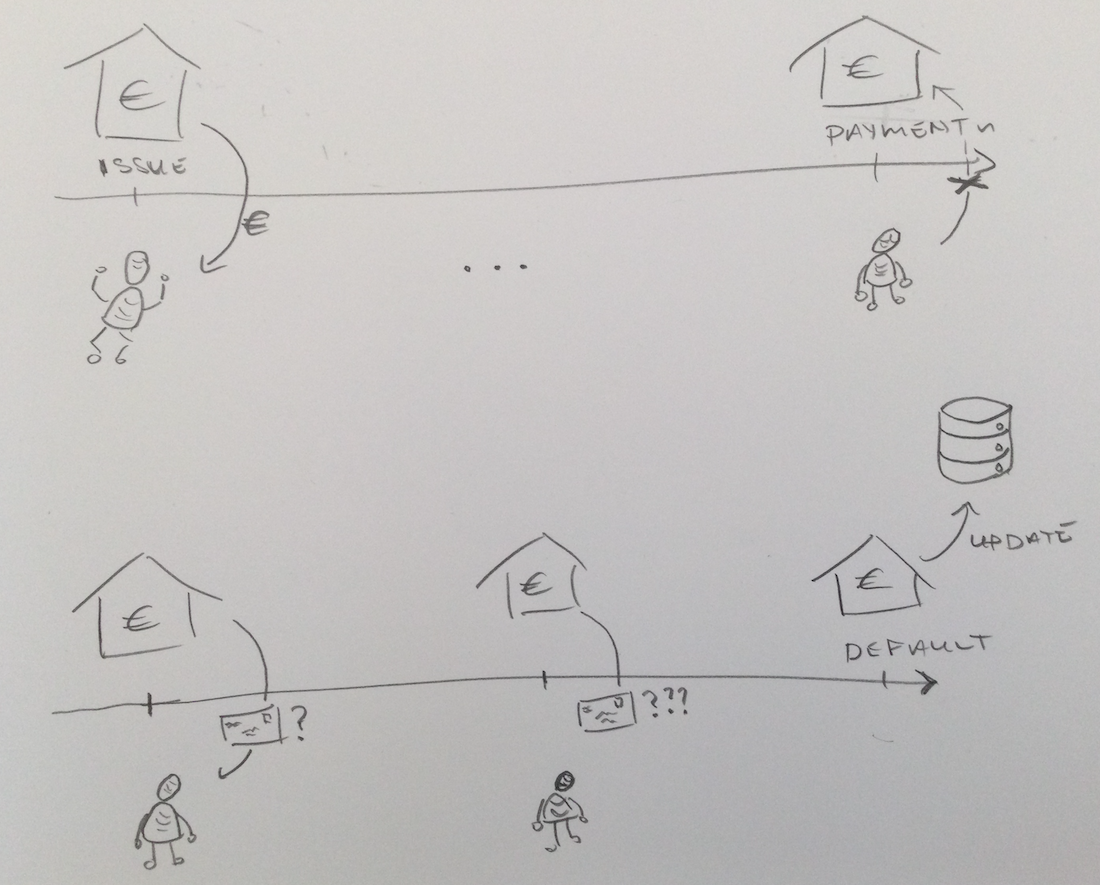
\includegraphics[height=0.6\textheight]{graphics/default-process-whole}
    \end{figure}

\end{frame}

\begin{frame}
    \frametitle{Manage Process Risk}
    \framesubtitle{Working with human nature in software development}
    \begin{center}
        
\includegraphics[height=0.35\textheight]{graphics/Codex_Aemilianensis}
        \end{center}
        Source: \url{https://commons.wikimedia.org/wiki/File:Codex_Aemilianensis.jpg}
    \begin{itemize}
    \item Agile: \href{https://agilemanifesto.org/}{agilemanifesto.org}
    \item Test Driven Development: \href{https://www.oreilly.com/library/view/test-driven-development/0321146530/}{Kent Beck, {\it Test Driven Development: By Example}}
    \item DevOps and MLOps: \href{https://landing.google.com/sre/books/}{Google's {\it Site Reliability Engineering}}
    \end{itemize}
\end{frame}

\begin{frame}
    \frametitle{Manage Process Risk}
    \framesubtitle{Isn't AI software different?}
    \begin{columns}[T] % align columns
        \begin{column}{.4\textwidth}
            \begin{center}
                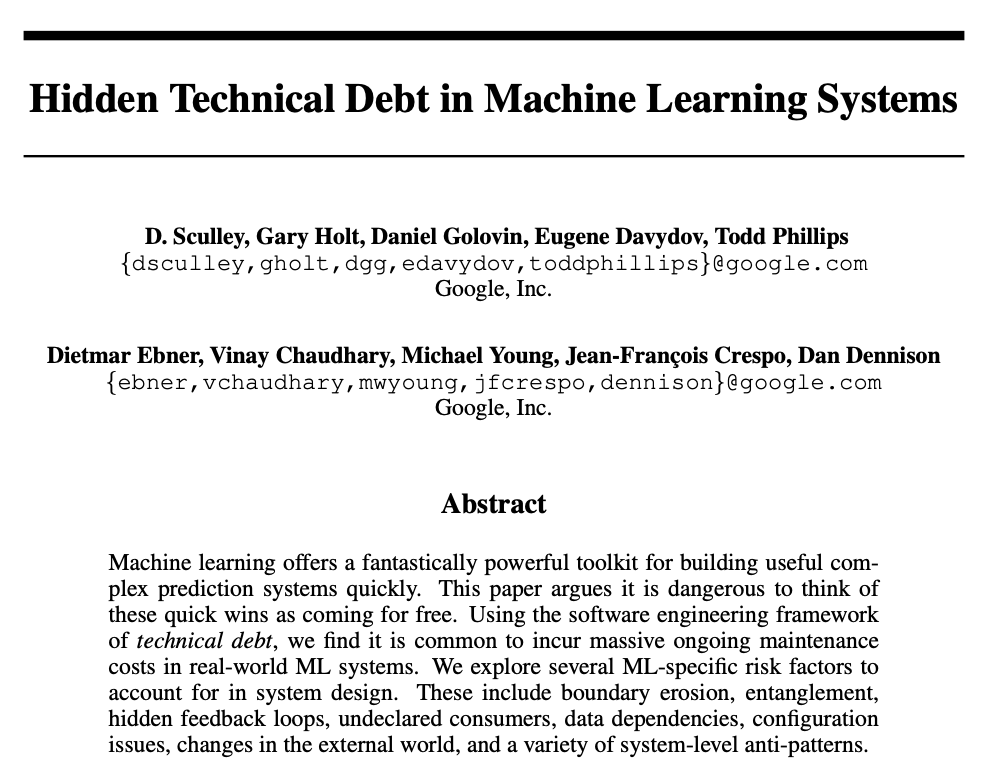
\includegraphics[height=0.35\textheight]{graphics/neurips-hidden-tech-debt}
            \end{center}
            Source: \href{https://proceedings.neurips.cc/paper/2015/hash/86df7dcfd896fcaf2674f757a2463eba-Abstract.html}{Neurips 2015, Hidden TechDebt in ML}
        \end{column}%
        \begin{column}{.4\textwidth}
            \begin{center}
                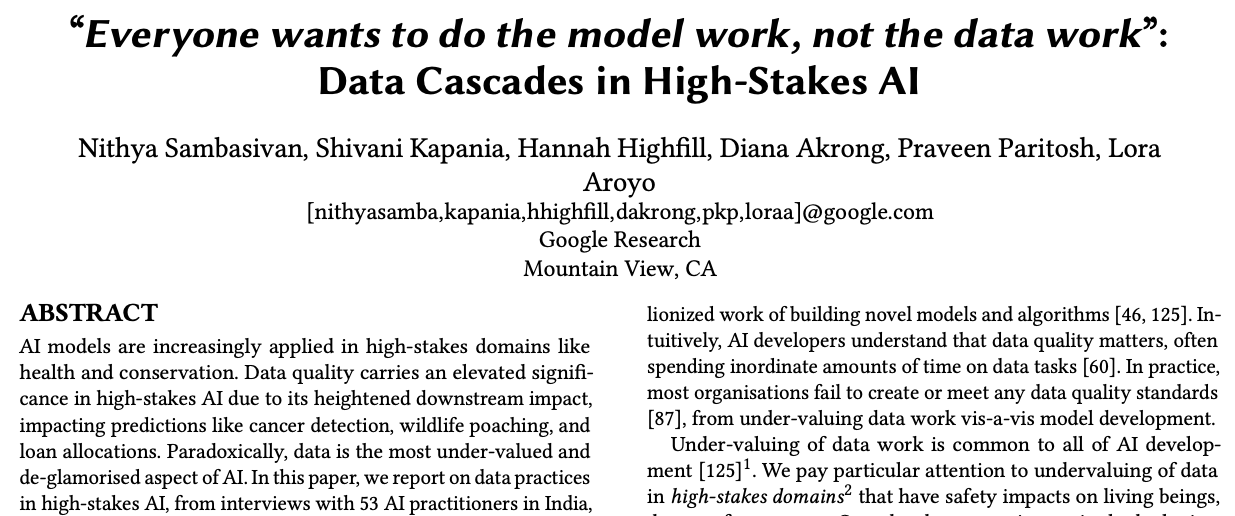
\includegraphics[height=0.25\textheight]{graphics/data-cascades}
            \end{center}
            Source: \href{https://nithyasambasivancom.files.wordpress.com/2021/01/sambasivan_cascades_chi2021.pdf}{Data Cascades in High-Stakes AI}
        \end{column}%
    \end{columns}

\end{frame}

\begin{frame}
    \frametitle{Manage Process Risk}
    \framesubtitle{Matching low-resolution buzzwords with high-resolution practice}

    \begin{block}{Continuous Integration, Continuous Delivery for Machine Learning}
        (Semi-)automated pipelines for development
        \begin{figure}[ht]
            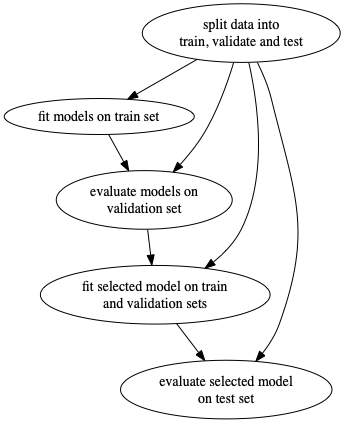
\includegraphics[height=0.5\textheight]{graphics/ml_pipeline}
        \end{figure}
        derived from \href{https://github.com/munichpavel/risk-ai-workshop/blob/main/risk_learning/model_selection/run-pipeline.py}{risk\_leaning/model\_selection/run-pipeline.py}
    \end{block}
\end{frame}

\begin{frame}
    \frametitle{Manage Process Risk}
    \framesubtitle{Matching low-resolution buzzwords with high-resolution practice}
    \begin{columns}[T]
        \begin{column}{0.48\textwidth}
            \begin{block}{Continuous Integration, Continuous Delivery for Machine Learning, II}
                (Semi-)automated pipelines for production
                \begin{figure}[ht]
                    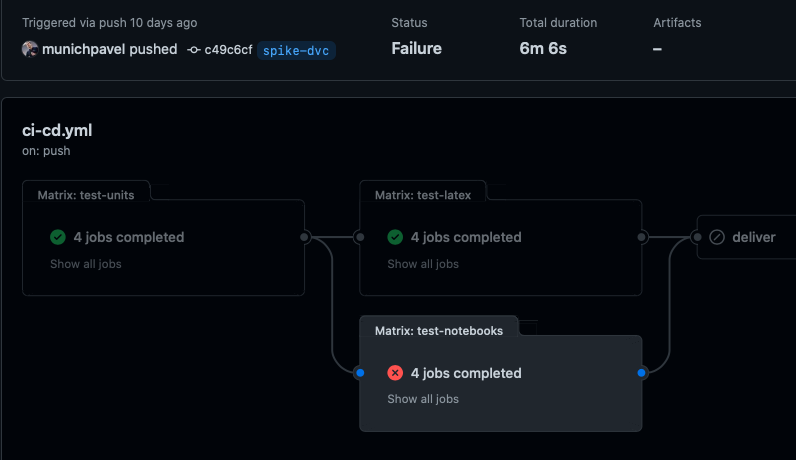
\includegraphics[height=0.25\textheight]{graphics/non-simple-ci-cd-pipeline}
                \end{figure}
                Source: \href{https://github.com/munichpavel/risk-ai-workshop/actions/runs/2038526473}{this repo's CI CD run \#37}; see \href{https://github.com/munichpavel/risk-ai-workshop/actions/runs/2084303272}{CI CD \#75} for a successful pipeline run, and the other \href{https://github.com/munichpavel/risk-ai-workshop/actions}{CI CD pipeline runs} for many other near-misses.
            \end{block}
        \end{column}
        \begin{column}{0.48\textwidth}
            \begin{block}{Version control}
                \href{https://git-scm.com/doc}{Git} (or cousin) for collaboration sanity and audit-trail
                \begin{figure}[ht]
                    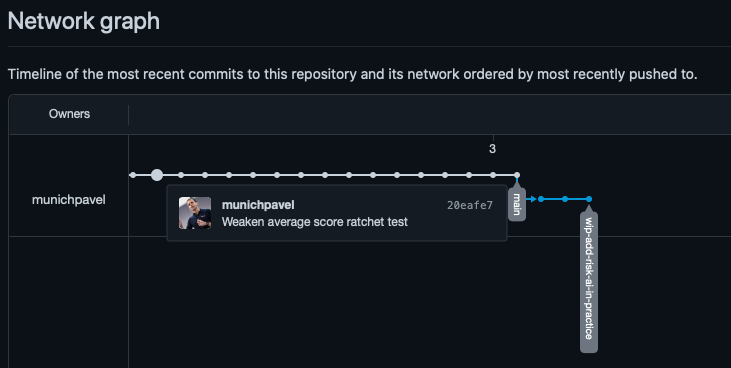
\includegraphics[height=0.25\textheight]{graphics/git-network-commit-graph}
                \end{figure}
                Source: \href{https://github.com/munichpavel/risk-ai-workshop/network}{This repo's GitHub commit graph}
            \end{block}
        \end{column}
    \end{columns}
\end{frame}

\begin{frame}{Wrapping up}
    \framesubtitle{Don't worry: AI won't replace you soon}
    \begin{columns}[T] % align columns
        \begin{column}{.40\textwidth}
            \begin{figure}[ht]
                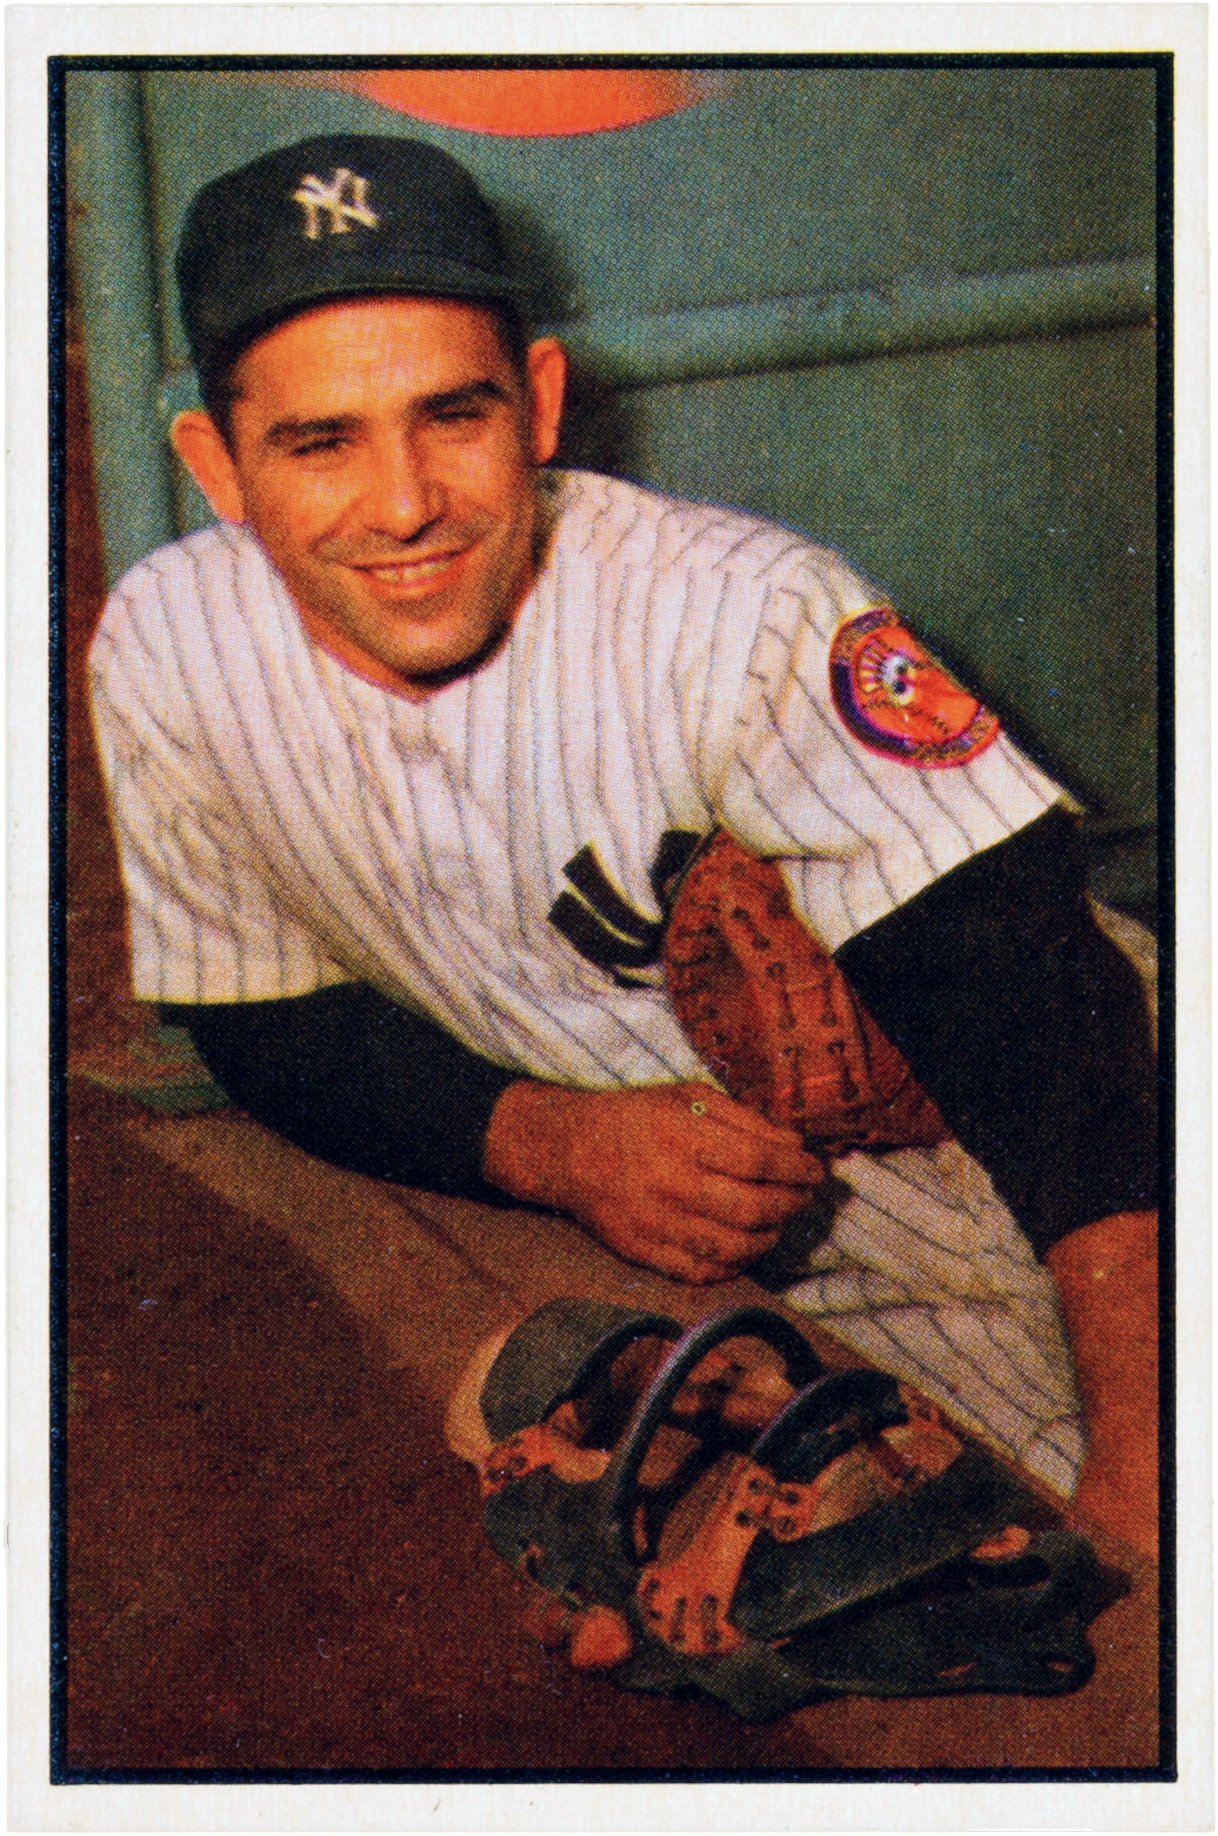
\includegraphics[height=0.4\textheight]{graphics/1953_Bowman_Yogi_Berra}
            \end{figure}
            \emph{In theory, there is no difference between theory and practice. \newline
            In practice, there is.}\newline
            Yogi Berra
        \end{column}
        \begin{column}{0.56\textwidth}%
                \begin{block}{$\rightarrow$ Risk is to managed, not eliminated}
            \end{block}
            \begin{block}{$\rightarrow$ Manage operational risk in AI by think deeply in practice}
                \ldots about the process and its data
                \newline
                \ldots about the algorithms you use
                \newline
                \ldots about potential impacts on society
            \end{block}
            \begin{block}{$\rightarrow$ Manage operational risk in AI by automating everything sensible}
            \end{block}
        \end{column}
    \end{columns}
\end{frame}

\end{document}